\chapter{Discussion}

This section discusses the results obtained from using sample-based metrics with possible interpretations. The best-performing model from the fine-tuning-based approach and feature-based approach is further evaluated on manually selected samples. Section \ref{quantitative_analysis} discusses a quantitative comparative analysis of language models and baselines with sample-based metrics. Section \ref{Qualitative_analysis} analyzes the quality of the best performing model from the fine-tuning-based approach and feature-based approach by evaluating some manually generated sentences.


\section{Quantitative analysis} \label{quantitative_analysis}
This section deals with quantitative analysis of language models and baselines using sample based metrics. Label based metrics and other significant properties are also discussed and compared in this analysis. 


Since it's important in our multi-label setup to identify whether a sample is a stereotype or anti-stereotype/unrelated, these categories must be ranked higher than others. Considering a case of partial matches with bias types categories (gender, ethnicity etc.) and excluding stereotype and anti-stereotype/unrelated categories might be a bit misleading. In this case, subset accuracy is simple, harsh, but a good measure as the exact match for the ground truth label is considered, thus giving equal importance to every label, including stereotype and anti-stereotype. Hence, subset accuracy is considered an important metric among the sample based metrics when doing quantitative analysis.
% Sample-based metrics were used to evaluate the performance of language models and baselines. Since it's important in our multi-label setup to identify whether a sample is a stereotype or anti-stereotype/unrelated, these categories must be ranked higher than others. Considering partial matches with bias types categories (gender, ethnicity etc.) and excluding stereotype and anti-stereotype/unrelated categories might be a bit misleading. In this case, subset accuracy is simple, harsh, but a good measure as the exact match for the ground truth label is considered, thus giving equal importance to every label, including stereotype and anti-stereotype. Hence, subset accuracy is considered an important metric among the sample based metrics when doing quantitative analysis. Other metrics such as label based metrics and  precision recall and f1-scores per class label are also being considered as parameters for quantitative analysis.

% \textbf{Test for synonyms...} on machine learning and language model to be done

\subsection{Evaluation of Language models}
Considering the first research question, i.e., how will different pre-trained language models impact the detection of stereotypes; different language models were trained and tested on a test set and evaluated using different evaluation metrics. These metrics reveal different perspectives of the result and will be discussed in this section. 

\begin{figure}[h!]
    \centering
    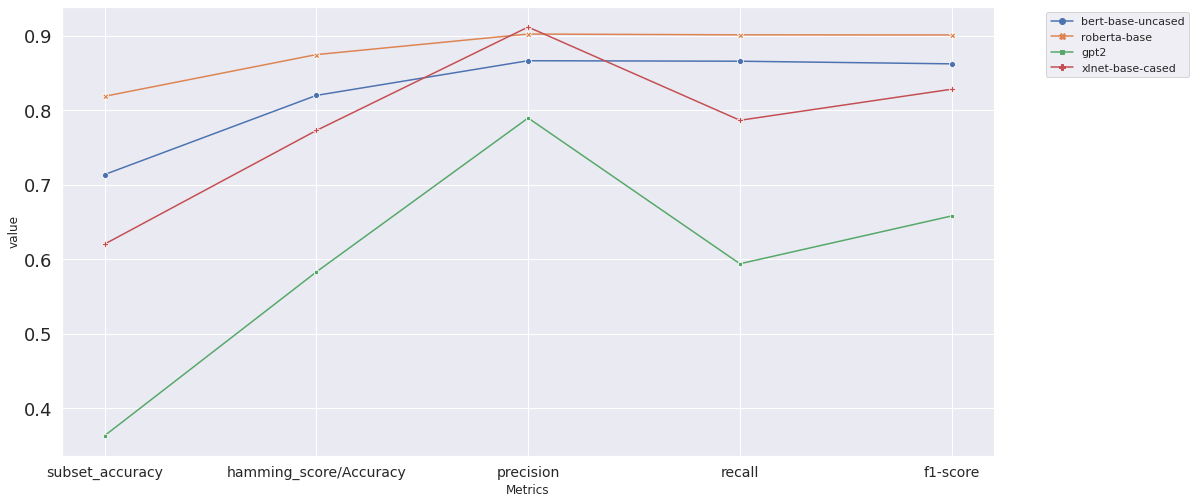
\includegraphics[width=1\textwidth]{thesis/figures/summary.png}
    \caption{Sample average results of language models }
    \label{fig:model_wise_group_LM}
\end{figure}
% A subset of sample-based metrics with similar scales have been compiled and can be seen in the figure \ref{fig:model_wise_group_LM}.
\subsubsection{Roberta}
Overall, Roberta is the best performing language model. Considering subset accuracy, roberta could achieve an accuracy of 81\%, which is 12.8\% more than the bert (next best to Roberta) and 40.2\% greater than the best performing baseline model (decision tree with tf\_idf). From the figure \ref{fig:model_wise_group_LM} it is clear that except for the sample average precision of xlnet, which is 1.04\% greater than Roberta, it is the best performing model among others. Coming to label-based measure \ref{LMreports} micro and macro average, it follows the same pattern that in the sample average results, where the precision of xlnet is slightly better but the recall, f1-score of roberta is highest for both the measures. The macro average f1-score is 0.69\% higher than sample average score. The micro average f1-score is score  1.04\% less than sample average f1-score. The label wise scores of language models can be found in the figure \ref{tab:Per-Label-precision-recall-f-measure}.The  f1-score of 'stereotype' class is 83.3\%, which is 8.85\% greater than bert 'stereotype' class f1-score and 13.17\% greater than xlnet 'stereotype' class f1-score. The f1-scores of stereotype and anti-stereotype on an average are 10 to 20\% lower when compared to scores of bias types (ethnicity, gender, profession, religion), which indicates that the classifier is better at identifying bias types. One of the characteristic properties of roberta are its hyperparameters used for training. The hyper-parameter search results of roberta \ref{tab:search_results} were different with higher number of epochs and a different learning rate, which might be one of the reasons for having high scores. Another significant property of roberta is its training data. Apart from the training data used for bert, it was trained on CC-News (English portion of Common crawl newsdataset, 76 GB), openWebText (web content extracted from URLs shared on Reddit with atleast three upvotes. 38GB). Since, its trained on Reddit which has several subreddits related to target terms in stereoset \cite{nadeem2020stereoset}, this might have some effect on the classification as the knowledge is being transferred. 

% \begin{itemize}
%     \item Roberta: The advantages of using transfer learning and language models is the robustness of the model apart from the effectiveness.
% \end{itemize}

\subsubsection{Bert}
Bert is the next best performing language model. As can be seen from the figure \ref{fig:model_wise_group_LM}, there is a marginal difference in the performance betweeen roberta and bert. The subset accuracy of bert is 71.37\% which is 13.08\% higher than xlnet and 12.8\% less than roberta. When compared to best performing baseline model (decision tree with tf\_idf), bert subset accuracy is 18.21\% higher. The sample average scores of roberta and bert vary by around 4.49\% for precision, recall, f1-score. Coming to label based metrics such as micro and macro average precision, recall and f-measure \ref{LMreports}; the micro  average f1-score is 1.33\% greater than sample average f1-score while macro average f1-score is 1.49\% less when compared to sample average f1-score.The label wise scores of language models can be found in the figure \ref{tab:Per-Label-precision-recall-f-measure}. As can be observed, the scores of bias categories are on an average 33.4\% higher than scores of stereotype and anti-stereotype. The f1-score of 'stereotype' class is 75.97\% while anti-stereotype is 63.45\% which is around 8 to 9\% less than roberta. The sample average scores of bert and roberta vary by 4\% which may be due to the fact that roberta was trained for 5 epochs while other models including bert was trained for 2 epochs. Since, roberta is an optimized version of bert, similar behaviour can be observed.

\subsubsection{Xlnet}
Xlnet language model has a subset accuracy of 62\% which is 13.08\% less than bert and 24.2\% less than roberta. As can be seen from the figure \ref{fig:model_wise_group_LM}, the precision of xlnet is higher than roberta by around 1.04\%, but the recall is significantly lower than roberta and bert. The reason for such high precision could be based on the language model architecture. As xlnet is a generalized autoregressive model which incorporates bidirectional context on the pure autoregressive model, an effect can be observed in the precision being very close to that of auto encoding models (bert and roberta) which also incorporate bidirectionality.  Coming to the label based metrics, micro macro average scores \ref{LMreports}, the scores show same trend as in sample average with no significant changes. The f1-score of 'stereotype' class is around 72.36 \% while 'anti-stereotype' class has 53.56\%.

\subsubsection{GPT-2}
GPT-2 is the worst performing model among language models. As can be seen from the figure \ref{fig:model_wise_group_LM} it has the lowest subset accuracy of 36.31\% when compared to other language models, and it's significantly lower than the best performing baseline (decision tree using \acrshort{tfidf}) by 60.75\%. The significant low performance might be due to language model architecture. 
% GPT-2 is purely autoregressive model trained for language modeling task and hence using it for text classification might be the reason. 
The sample average precision is 78.97\% which is 9.7\% lower than bert precision, but recall is significantly lower (45.78\% than bert) and  (32.4\% than xlnet) which leads to a f1-score of 65.82\% (13.19\% lower than decision tree using \acrshort{tfidf}). Coming to label based metrics, micro and macro average f1-score remain almost the same. The f1-score of 'stereotype' is 47.45 \% while of 'anti-stereotype' is 20.7\% which are the lowest scores among others. 


\subsection{Evaluation of Baselines}
% \begin{figure}[h!]
%     \centering
%     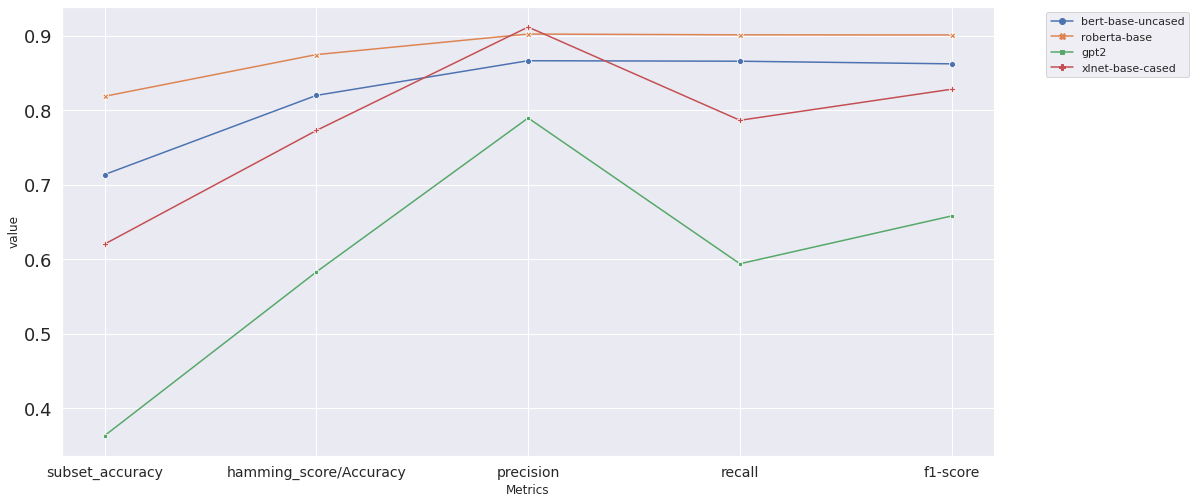
\includegraphics[width=1\textwidth]{thesis/figures/summary.png}
%     \caption{Sample average metrics summary results of language models }
%     \label{fig:model_wise_group_LM}
% \end{figure}
\begin{figure}[h!]
    \centering
    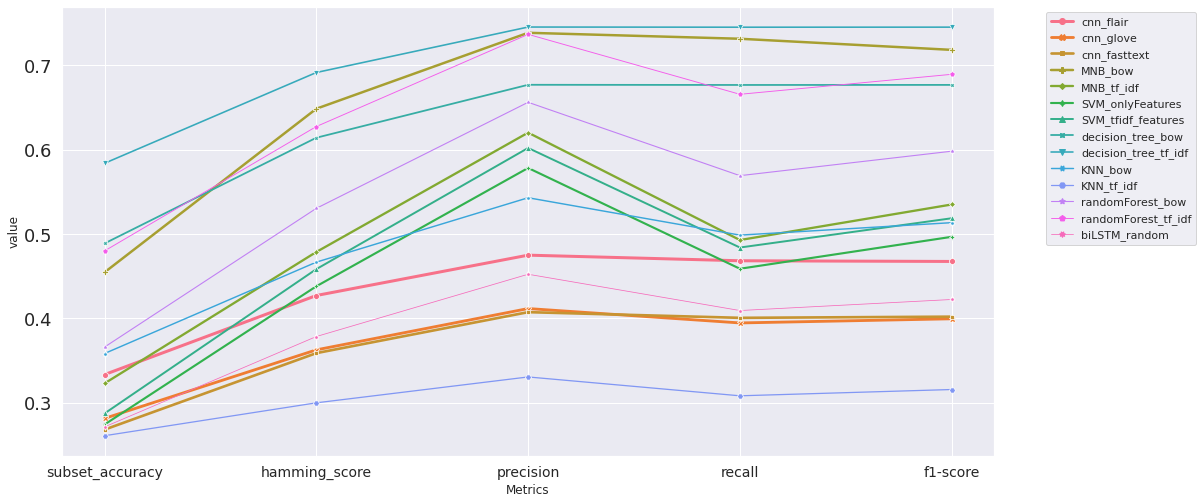
\includegraphics[width=1\textwidth]{thesis/figures/Baslines.png}
    \caption{Sample average metrics summary results of baseline models }
    \label{fig:model_wise_group_baseline}
\end{figure}
% \begin{itemize}
%     \item MNB and decision tree: Through training these models is far cost-effective, the robustness of the model remains an issue. 
%     \item The results on the test set states that these machine learning models are performing well on explicit features, but when tested with random samples, it might fail miserably. 
% \end{itemize}
Figure \ref{fig:model_wise_group_baseline} shows a cumulative view of different baselines tested. Out of the many, decision tree using \acrshort{tfidf} is the best performing model followed by multinomial naive Bayes with bag of words features and random forest with tf\_idf features. These models have achieved a significant performance when compared to deep learning models with pre-trained word embeddings. A pattern that could be observed is that tree based models have outperformed other models. Features such as bag of words with uni-gram features and tf\_idf could outperform pre-trained word embedding models including flair, which is a contextual word embedding model.  


\section{Qualitative analysis} \label{Qualitative_analysis}
\begin{itemize}
    \item Interpretation of results and Selecting best performing model 
    \item Best performing model discussion with manual sentences (Test cases ) 
    \begin{itemize}
        \item Effectiveness (Metrics)
        \item Efficiency (time)
        \item Test Explicit(Associations to stereo attribute) and implicit (Analogies) stereotypes
        \begin{itemize}
            \item Explicit stereotypes : Overt expression of target with attribute, e.g. target : African, stereotypic attribute : good at running
            \item Implicit stereotypes : Subtle expression of stereotypes where the target is an instance of target and where the attribute may be synonymous as well
            e.g. Target : African name, stereotypic attribute :  good at running 
        \end{itemize} 
        \item Test for explicit stereotypical bias statements  (stereotypical, anti-stereotypical and unrelated)
        \item Test by changing target other than the provided in dataset 
        \item Manual evaluation with respect to selected arguments (IBM dataset) and analysis with respect to user study 
    \end{itemize}
\end{itemize}